\documentclass[french, 12pt]{article}%


\usepackage[T1]{fontenc}
\usepackage[utf8]{inputenc}
\usepackage[french]{babel}

\usepackage{textcomp}

\usepackage[official]{eurosym}

\usepackage{appendix}
\usepackage{pdfpages}

%%%%%%%%%%%%%%%%%%%%%%%%%%%%%%%%%%%%%%%%%%%%%%%%%%%%%%%%%
\newcommand{\itemE}{\item[$\bullet$]}

\newcommand{\titreSeq}{Installation de l'environnement}
\newcommand{\lycee}{Académie rennes}
\newcommand{\classSeq}{CIEL }
\newcommand{\matiereSeq}{IR}      
\newcommand{\numSeq}{Cyber}
\newcommand{\numAct}{01}
\newcommand{\objSeance}{Proposer et mettre en place une plateforme de tests}

\newcommand{\moySeq}{\begin{itemize}	
\itemE VM Kali
\itemE VM serveurCyber
\itemE VM Pfsense
\end{itemize}}


\newcommand{\paraL}[1]{\tiny\noindent\rule{1.0\linewidth}{0.5pt}\paragraph*{#1}\  \normalsize}


\newcommand{\compSeq}{\begin{itemize}
\item  
\end{itemize}}
%%%%%%%%%%%%%%%%%%%%%%%%%%%%%%%%%%%%%%%%%%%%%%%%%%%%%%%%%%

%%%%%%%%%%%%%%%%%%%%%%%%%%%%%%%%%%%%%%%%%%%%%%%%%%%%%%%%
%%%%Algo
\usepackage[linesnumbered, french]{algorithm2e}
\SetKwFor{For}{Pour}{faire}{fin}
\SetKwFor{While}{Tant que}{faire}{fin}%
\SetKw{KwTo}{?}
\SetKw{KwPas}{par pas de}
\SetKw{KwRet}{Retourne}
\SetKwProg{Fn}{Fonction }{ arguments }{fin}
\SetKwRepeat{Repeat}{Répéter}{jusqu'?}%
\SetKwIF{If}{ElseIf}{Else}{Si}{alors}{Sinon si}{Sinon}{Fin}


\usepackage{listings} %%%%Présenration code source
\lstset{language=C++,
    %numbers=left,
   %stepnumber=1,
    showstringspaces=false,
    tabsize=1,
    breaklines=true,
    breakatwhitespace=false,
    basicstyle=\footnotesize,
    keywordstyle=\color{blue}\footnotesize,
    stringstyle=\color{red}\footnotesize,
    commentstyle=\color{magenta}\footnotesize,
    morecomment=[l][\color{magenta}]{\#}
    }
\lstdefinestyle{commande}{
  basicstyle=\ttfamily\footnotesize,
  keywordstyle=\color{blue},
  commentstyle=\color{gray},
  %numbers=left,
  %numberstyle=\tiny\color{gray},
  numbersep=5pt,
  breaklines=true,
  frame=single,
  backgroundcolor=\color{lightgray!10}
  %captionpos=b,
  %caption=\lstname  
}

%\usepackage[T1]{fontenc}

\newcommand{\itemB}{\item[$\Box$]}
% Margins
\topmargin=-0.45in
\evensidemargin=0in
\oddsidemargin=0in
\textwidth=6.5in
\textheight=9.0in
\headsep=0.25in 


\linespread{1.1} 
\usepackage{amsmath}%
\usepackage{amsfonts}%
\usepackage{amssymb}%
\usepackage{graphicx}
\usepackage{lastpage}
\usepackage{enumitem}

%\usepackage[T1]{fontenc}    
\usepackage{multirow}
\usepackage{lscape}
\usepackage[colorlinks = true,
            linkcolor = blue,
            urlcolor  = blue,
            citecolor = blue,
            anchorcolor = blue]{hyperref}
\usepackage{array}
\usepackage{mwe}
%-------------------------------------------
\newtheorem{theorem}{Theorem}
\newtheorem{summary}[theorem]{Summary}
\newenvironment{proof}[1][Proof]{\textbf{#1.} }{\ \rule{0.5em}{0.5em}}



\usepackage{xcolor}

\usepackage{colortbl}
\definecolor{vert_capet}{RGB}{191,255,191}	
\definecolor{bleu_snir}{RGB}{101,191,179}	
\setlength{\doublerulesep}{\arrayrulewidth}
%-------------------------------------------
%%%%%%%%%%%%%%%%%%%%%%%%%%%%%%%%%%%%%%%%%%%%%
\usepackage[framemethod=tikz]{mdframed}
\usepackage{tikz, xcolor, lipsum}
\makeatletter
\mdfsetup{skipabove=\topskip,skipbelow=\topskip}

\tikzset{titre_bleu_snir/.style =
	{draw=bleu_snir, line width=1.5pt, fill=white,
	rectangle, rounded corners, right,minimum height=2em}}
\newcommand{\titreencadre}{Titre}
\makeatletter
\mdfdefinestyle{encadrestyle}{%
	linewidth=1.5pt,roundcorner=5pt,linecolor=bleu_snir,
	apptotikzsetting={\tikzset{mdfbackground/.append style ={%
		fill=white}}},
	frametitlefont=\bfseries,
	singleextra={%
		\node[titre_bleu_snir,xshift=2em] at (P-|O) %
			{~\mdf@frametitlefont{\titreencadre}\hbox{~}};},
	firstextra={%
		\node[titre_bleu_snir,xshift=2em] at (P-|O) %
		{~\mdf@frametitlefont{\titreencadre}\hbox{~}};},
	}
\mdfdefinestyle{encadresanstitrestyle}{%
	linewidth=1.5pt,roundcorner=5pt,linecolor=bleu_snir
	apptotikzsetting={\tikzset{mdfbackground/.append style ={%
		fill=yellow!20}}},
	}

\newenvironment{encadre}[1]{\renewcommand{\titreencadre}{#1}
	\begin{mdframed}[style=encadrestyle]
	\vspace{0.5\baselineskip}
	}{%
	\end{mdframed}}

\newenvironment{encadresanstitre}{
	\begin{mdframed}[style=encadresanstitrestyle]
	}{%
	\end{mdframed}}
\makeatother
\usepackage{colortbl}
\definecolor{vert_capet}{RGB}{191,255,191}	
\definecolor{bleu_snir}{RGB}{101,191,179}	
\setlength{\doublerulesep}{\arrayrulewidth}
%-------------------------------------------
\usepackage{comment}
%%%%%%%%%%%%%%%%%%%%%%%%%%%%%%%
\newif\ifPROF

%\def\PourProf{0}
\ifdefined\PourProf
  \PROFtrue
  \newenvironment{corr}{\begingroup \color{red}}{\normalcolor \endgroup}
\else
  \PROFfalse
  \newenvironment{corr}{\begingroup \color{white}}{\normalcolor \endgroup}
\fi

%\PROFtrue

%%%%%%%%%%%%%%%%%%%%%%%%%%%%%%%%%%%%




%%%Note et pied de page
\usepackage{fancybox}
\usepackage{fancyhdr}
\usepackage[a4paper,margin=2.5cm,bottom=2cm,headheight=2cm]{geometry}
\pagestyle{fancy}
\fancyhead[R]{
\includegraphics[scale=0.3]{logo_CIEL.png}}
\fancyhead[C]{Prénom}
\fancyhead[L]{Nom}
\fancyfoot[C]{Page \thepage/\pageref{LastPage}}
\fancyfoot[L]{\classSeq ~\matiereSeq}
\fancyfoot[R]{Formation \numSeq  ~ Act \numAct}
\renewcommand{\headrulewidth}{1pt}
%%%Note et pied de page 



\begin{document}
\lstset{basicstyle = \ttfamily,columns=fullflexible}

\title{\titreSeq\\
 \includegraphics[scale=0.5]{logo_sti2d.png}\\
}
\author{\lycee}
\date{}%\today}
%\maketitle

\noindent\begin{tabular}{!{\vrule width 1.5pt}m{0.7\linewidth}!{\vrule width 1.5pt}m{0.2\linewidth}!{\vrule width 1.5pt}}
\hline\hline
\cellcolor{green!25}
\begin{center}
	\Large\textbf{\titreSeq}  
\end{center}
  & 

\begin{minipage}{1.0\linewidth}
  \vspace*{0.1cm} 
\centering
\includegraphics[scale=0.2]{logo_lycee.jpg}

{\tiny\today}
  \vspace*{0.1cm} 
\end{minipage}\\ \hline\hline

\multicolumn{2}{!{\vrule width 1.5pt}l!{\vrule width 1.5pt}}{
\begin{minipage}{14cm}
\vspace*{0.1cm} 
\textbf{Objectif} : \objSeance
\vspace*{0.1cm} 
\end{minipage}} \\ \hline\hline

\multicolumn{2}{!{\vrule width 1.5pt}l!{\vrule width 1.5pt}}{
\begin{minipage}{14cm}
\vspace*{0.1cm} 
\textbf{Moyens} : 
\moySeq
\vspace*{0.1cm} 
\end{minipage}} \\ \hline\hline
%
%\multicolumn{2}{!{\vrule width 1.5pt}l!{\vrule width 1.5pt}}{
%\begin{minipage}{14cm}
%\vspace*{0.1cm}
%\tiny
%Compétences attendues :
%\compSeq
%\vspace*{0.1cm}
%\end{minipage}}
%\normalsize \\ \hline\hline
\end{tabular}

%%%%%%%%%%%%%%%%%%%%%%%%%%%%%%%%%%%%%%%%%%%%%%%%%%%%%%%%%%%%%%%%%%%%%%%%%%%%%%%%
\section{Dépot}

Les énoncés sont présents sur : 
\url{https://ciel-broceliande.myasustor.com/}
avec
\begin{itemize}
\itemE Login : \verb?formationCyber?
\itemE Mot de passe : \verb?acRennes!!2025?
\end{itemize}


\begin{minipage}{0.65\linewidth}
Pour les besoins de la formation, les dépôts GitHub présentent dans le tableau ci-dessous vont être utilisés.
\end{minipage}
\begin{minipage}{0.34\linewidth}
\begin{center}

\includegraphics[scale=0.25]{./ressource/logoGit.jpeg}
\end{center}
\end{minipage}




\begin{encadre}{GitHub }
Plateforme web de gestion de code source qui permet d'héberger, collaborer et versionner des projets via Git. Elle est très efficace pour le travail en équipe et pour l’intégration et le déploiement continus.
\end{encadre}

\footnotesize
\begin{tabular}{|>{\raggedright\arraybackslash}p{4cm}|
                >{\raggedright\arraybackslash}p{5cm}|
                >{\raggedright\arraybackslash}p{5cm}|}
\hline
\rowcolor{vert_capet} \textbf{Activités} & \textbf{Description} & \textbf{URL GitHub} \\
\hline

\begin{minipage}{\linewidth}
\vspace{0.2cm}
\begin{itemize}
  \itemE \texttt{act02-https}
  \itemE \texttt{act03-monitoring}
  \itemE \texttt{act04-SNMP\_P}
  \itemE \texttt{02-wifi}
\end{itemize}\vspace{0.2cm}
\end{minipage}
& Serveur temperature + client python\&ESP32 + falsification client
& \url{https://github.com/PierreViland/serveurSimpleIot.git} \\
\hline

\begin{minipage}{\linewidth}
\begin{itemize}
  \itemE Toutes
\end{itemize}
\end{minipage}
& Serveur LEMP et LAMP HTTP/HTTPS 
& \url{https://github.com/PierreViland/00-serveurLemp.git} \\
\hline

\begin{minipage}{\linewidth}
\begin{itemize}
  \itemE \texttt{act02-https}
\end{itemize}
\end{minipage}
& Exemple phishing avec certificat Let's Encrypt 
& \url{https://github.com/PierreViland/httpsPhishingExemple.git} \\
\hline

\begin{minipage}{\linewidth}\vspace{0.2cm}
\begin{itemize}
  \itemE \texttt{act03-monitoring}
  \itemE \texttt{act04-SNMP\_P}
  \itemE \texttt{act05-gestionLog}
\end{itemize}\vspace{0.2cm}
\end{minipage}
& Monitoring stack + Analyse de logs 
& \url{https://github.com/PierreViland/monitoringPV.git} \\
\hline

\begin{minipage}{\linewidth}
\begin{itemize}
  \itemE \texttt{act04-SNMP\_P}
\end{itemize}
\end{minipage}
& Zabbix 
& \url{https://github.com/akmalovaa/zabbix-docker} \\
\hline

\begin{minipage}{\linewidth}
\begin{itemize}
  \itemE Bonus
\end{itemize}
\end{minipage}
& Source \LaTeX{} des documents + workflow de déploiement 
& \url{https://github.com/PierreViland/formationCyber2025.git} \\
\hline
\end{tabular}
\normalsize

\begin{minipage}{0.49\linewidth}
\paragraph{Les ressources pour l'attaque et la protection Wifi} sont aussi déposé est dans les répertoires \verb?ressource_eleve? correspondant à l'énoncé de l'activité. 

\end{minipage}
\begin{minipage}{0.49\linewidth}
\begin{center}
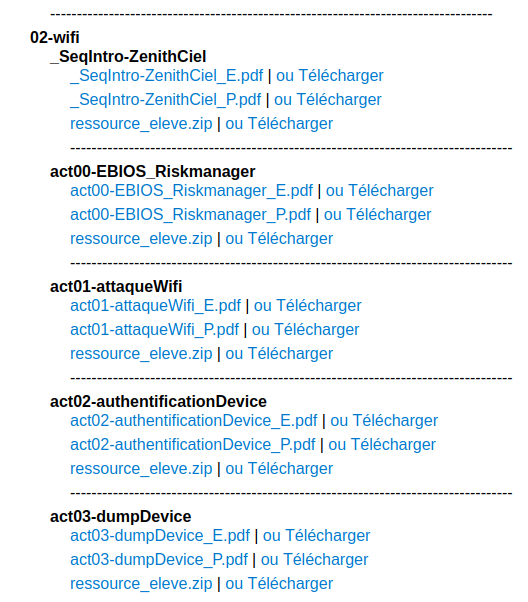
\includegraphics[scale=0.4]{./ressource/ressourceEleve}
\end{center}
\end{minipage}





\section{Système} 

Dans le cadre de la formation, nous allons reproduire les services et les éléments de la topologie réseau présentée ci-dessous, mais pas tous en même temps. Leur mise en place se fera progressivement, en fonction des activités.

\begin{center}
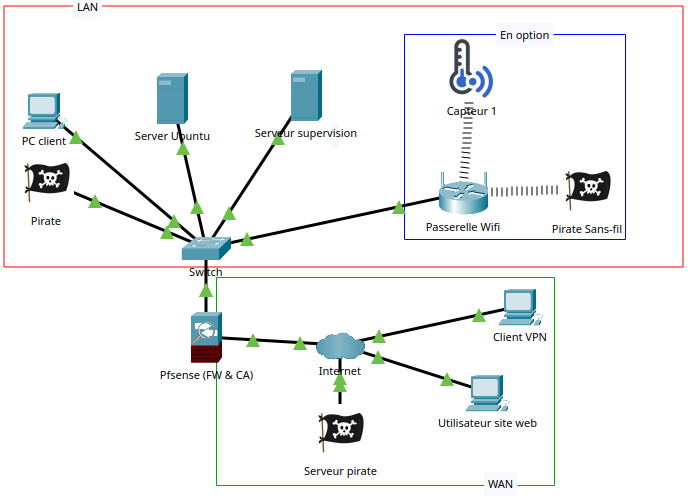
\includegraphics[scale=0.7]{./ressource/environnement.png}
\end{center}
avec : 
\begin{itemize}
\itemE \verb?Serveur Web? : contient des sites de tests, accessibles en http ou en https. 
\itemE Les \verb?pirates? : Machine simulant un pirate
\itemE \verb?Serveur supervision? : Machine ayant des services pour la centralisation des logs et la supervision des appareils et des services. 
\itemE \verb?SIEM? : Machine contenant un système de gestion des informations et des événements de sécurité (SIEM)
\itemE \verb?FW & CA? : Pare-feu faisant fonction d'autorité de certification (CA)
\end{itemize}

\paragraph{Remarque :} il aurait été plus judicieux de mettre le serveur dans une DMZ mais ce n'est pas le sujet de l'activité.  


\paragraph{Pour la majorité des activités proposées}n les manipulations peuvent être réalisées sur n'importe quel système d'exploitation, à condition que les éléments suivants soient installés :
\begin{itemize}
  \itemE \textbf{Docker}
  \itemE un \textbf{interpréteur Python}
\end{itemize}

Les sections ci-dessous présentent l’installation des environnements Ubuntu et pfSense, sur lesquels une partie des activités a été testée. Il n'est pas obligatoire d'utiliser le même type d'environnement. 



\section{Serveur web sur Ubuntu}

\
\begin{minipage}{0.6\linewidth}
Le serveur Ubuntu est basé sur la même VM que le serveur Cyber utilisé durant la précédente formation. Le disque de cette VM est présent dans les ressources et est nommé : \verb? ServeurCyber.vmdk? 

\end{minipage}
\begin{minipage}{0.39\linewidth}
\begin{center}

\includegraphics[scale=0.3]{./ressource/serveurUbuntu.jpeg}
\end{center}
\end{minipage}


\vspace{0.5cm}
\begin{lstlisting}[style=commande]
$lsb_release -a
No LSB modules are available.
Distributor ID:	Ubuntu
Description:	Ubuntu 22.04.5 LTS
Release:	22.04
Codename:	jammy
\end{lstlisting}


\begin{enumerate}
\item A partir de ce disque et avec Oracle Virtual box, créer une nouvelle machine virtuelle intégrée au LAN (Mode Bridge). La configuration réseau doit être en \textbf{mode promiscuité}.

\begin{center}
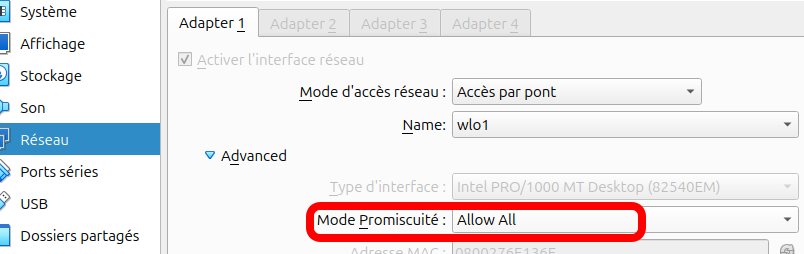
\includegraphics[scale=0.4]{./ressource/modeProm.png}
\end{center}
Cela va permettre de : 
	\begin{itemize}
	\itemE Sniffer le trafic réseau entre l'hôte et une VM (par exemple avec Wireshark)
	\end{itemize}
	
Le nom de l'interface réseau (dans l'image au-dessus \verb?Name wlo1?) dépend du nom de votre carte réseau.	

\item L'adressage IP est statique (possibilité de la mettre en dynamique). Elle vous sera donnée durant l'installation de vos machines. Pour la changer, il faut ouvrir le fichier \verb?00-installer-config.yaml? présent dans \verb?/etc/netplan:?
	\begin{lstlisting}[style=commande]
vi /etc/netplan/00-installer-config.yaml
\end{lstlisting}
Ensuite, effectuer les modifications souhaitées : 
	\begin{lstlisting}[style=commande]
network:
  version: 2
  renderer: networkd  
  ethernets:
    enp0s3:
      dhcp4: no  
      addresses:
       - 192.168.1.30/24
      routes:
        - to: default
          via: 192.168.1.1
      nameservers:
       addresses: [8.8.8.8, 1.1.1.1]

\end{lstlisting}


Il faut ensuite appliquer les modifications
\begin{lstlisting}[style=commande]
sudo netplan apply 
\end{lstlisting}



\item Les identifiants administrateurs de cette VM sont : 
	\begin{itemize}
	\itemE Login : \verb?pviland?
	\itemE Mot de passe : \verb?choupette?
	\end{itemize}

\item Il faut s'assurer que tous les containers soient stoppés et supprimés,  pour cela, il faut exécuter les commandes suivantes  : 
\begin{lstlisting}[style=commande]
root@serveurCyber:/home/pviland/monitoringPV/01-stackMonitoring# sudo su
root@serveurCyber:/home/pviland/monitoringPV/01-stackMonitoring# docker stop $(docker ps -q) && docker rm $(docker ps -aq)

\end{lstlisting}

\item Dans le répertoire de votre choix, cloner le dépôt contenant le serveur Web présent \href{https://github.com/PierreViland/00-serveurLemp.git}{https://github.com/PierreViland/00-serveurLemp.git}: 

	\begin{lstlisting}[style=commande]
pviland@serveurCyber:git clone https://github.com/PierreViland/00-serveurLemp.git
\end{lstlisting}
	
\end{enumerate}


\paragraph{Vérification de l'accès au dépôt et fonctionnement des containers}

\begin{enumerate}[resume]


\item Se placer dans le répertoire \verb?~/00-serveurLemp? et dans la branche  \verb?main? du dépôt git, créer et lancer les containers \footnote{Un document nommé \texttt{r01-dockerPresentation\_P.pdf}  est présent en ressource. Il présente le principe des dockers et donne les commandes de base}. 


\begin{lstlisting}[style=commande]
pviland@serveurCyber:~$ cd 00-serveurLemp/
pviland@serveurCyber:~/00-serveurLemp$ sudo docker compose up -d
[+] Running 5/5
  Network 00-serveurlemp_mynet  Created 0.2s
  Container mysqlPV             Started 2.1s
  Container phpmyadminPV        Started 1.9s
  Container phpPV               Started 3.5s
  Container nginxPV             Started 4.9s
\end{lstlisting}

\item Sur une machine de votre choix et le navigateur de votre choix, vérifier si le site est opérationnel. ATTENTION : il n'est pas encore sécurisé.

\begin{center}
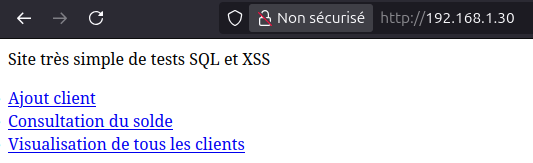
\includegraphics[scale=0.5]{./ressource/exServeurNonsecur.png}
\end{center}

\end{enumerate}

\paragraph{Si vous avez accès au site, vous avez un environnement de travail opérationnel}

\section{Pfsense}

Pfsense est un système d'exploitation basé sur FreeBsd conçu principalement pour servir de pare-feu. 

\begin{center}

\includegraphics[scale=0.4]{./ressource/pfsenseLogo}
\end{center}

En plus des fonctionnalités attendus par un pare-feu (filtrage, VPN, NAT, IDS/IPS, portail captif, ...), il peut permettre de gérer de manière très simple les certificats. La version de pfsense utilisée est : 
\begin{center}
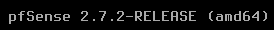
\includegraphics[scale=0.7]{./ressource/versionPfsense}
\end{center}


\paragraph{L'installation d'une machine virtuelle Pfsense} est détaillée en annexe \ref{lbl_pfsense}.  Pfsense ne sera pas utilisé comme pare-feu mais comme \textbf{autorité de certification}.  Ainsi, une subtilité dans l'installation est exploitée. Il n'est en effet pas nécessaire d'avoir les deux interfaces réseau opérationnelles en même temps. 
\begin{itemize}
\itemE Pour l'installation, seul le port WAN du pare-feu est connecté au réseau (avec internet). Le port LAN n'est pas connecté.
\itemE Une fois l'installation terminée, le port WAN est déconnecté. Le port LAN est connecté au réseau
\end{itemize}

\begin{center}
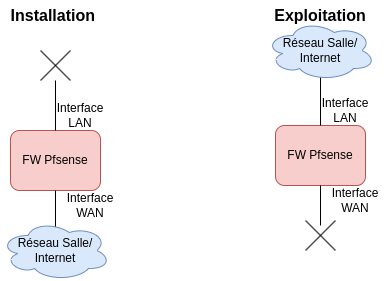
\includegraphics[scale=0.7]{./ressource/installPfense.png}
\end{center}

Ainsi, l'interface d'administration de Pfsense est accessible depuis votre LAN sans avoir à gérer des règles de filtrage. Pour tester son fonctionnement, il suffit d'aller sur la page de connexion de Pfsense via l'interface web: 


\begin{center}
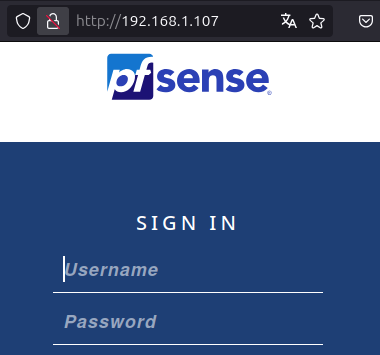
\includegraphics[scale=0.7]{./ressource/pfsenseLog}
\end{center}

Les identifiants sont  : 
\begin{itemize}
\itemE login : \verb?admin?
\itemE mot de passe : \verb?pfsense?
\end{itemize}


\begin{center}
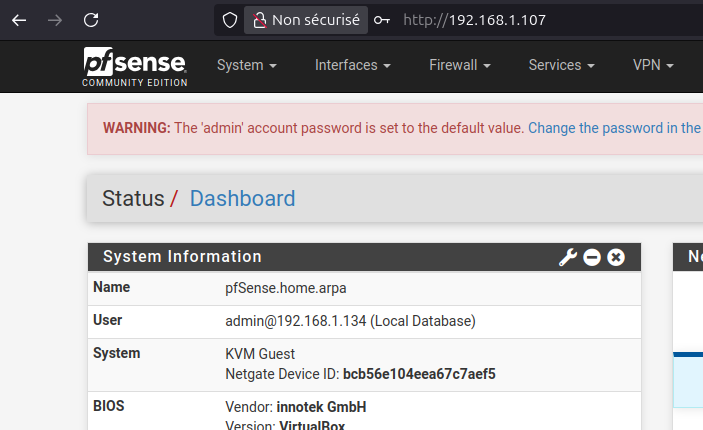
\includegraphics[scale=0.7]{./ressource/pfsenseIndex}
\end{center}

Vous avez maintenant un environnement opérationnel 
%%%%%%%%%%%%%%%%%%%%%%%%%%%%%%%%%%%%%%%%%%%%%%ANNEXE


\section{Kali Linux}
\begin{minipage}{0.6\linewidth}
Pour rappel : 
\begin{itemize}
\itemE \verb?Kali? est une distribution spécialisée dans le pentest et la cybersécurité. Toutes les informations se trouvent sur  \href{https://www.kali.org/}{leur site}. \verb?Kali? n'est pas la seule distribution spécialisée dans la cybersécurité. On peut citer \verb?Arch Linux?.
\itemE Les identifiants de l'un des comptes présents sur la VM sont: 
	\begin{itemize}
	\item[+] Login : \verb?kali?
	\item[+] Mot de passe : \verb?kali?
\end{itemize}	 
\end{itemize}
\end{minipage}
\begin{minipage}{0.4\linewidth}
\begin{center}

\includegraphics[scale=0.4]{./ressource/logoKali}
\end{center}
\end{minipage}
\vspace{0.25cm}

La machine virtuelle nommée \verb?Kali? est présente dans le répertoire \verb?ressource_eleve/VM/?. La version utilisée est la suivante :


\begin{lstlisting}[style=commande]
$lsb_release -a

No LSB modules are available.
Distributor ID: Kali
Description:    Kali GNU/Linux Rolling
Release:        2024.4
Codename:       kali-rolling
\end{lstlisting}
\section{Conclusion}

Dans cette partie, nous avons mis en place l'environnement de travail. Dans la prochaine activité, il va falloir la sécuriser.

\clearpage
\appendix
\section{Installation de pfsense}
\label{lbl_pfsense}
Pour l'installation de Pfsense, il suffit de suivre les directive ci-dessous : 

\begin{enumerate}
\item Créer un machine virtuelle sous VirtualBox en prenant l'iso nommé : 

\verb?netgate-installer-amd64.iso? présent en ressource.
\end{enumerate}

\begin{center}
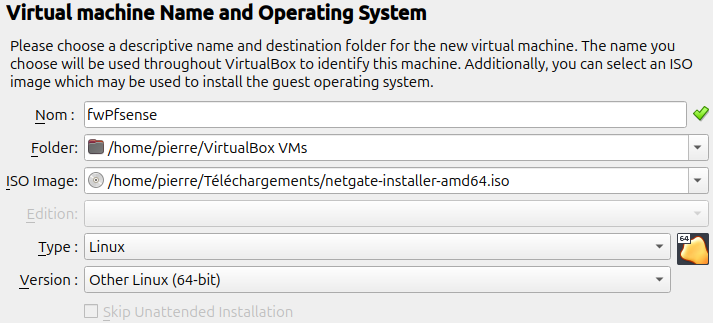
\includegraphics[scale=0.5]{./ressource/VM_Create_1.png}
\end{center}

\begin{enumerate}[resume]
\item La configuration matérielle minimale doit être : 
\end{enumerate}

\begin{center}
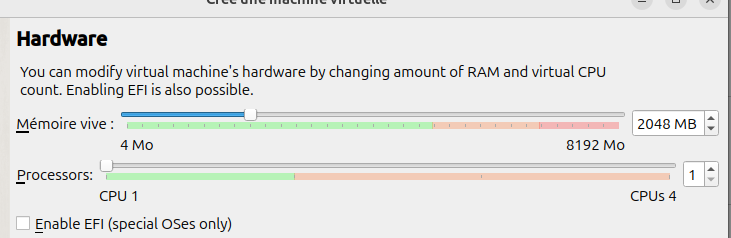
\includegraphics[scale=0.5]{./ressource/VM_Create_2.png}
\end{center}

\begin{enumerate}[resume]
\item Il n'est pas nécessaire d'avoir un espace disque important : 
\end{enumerate}

\begin{center}
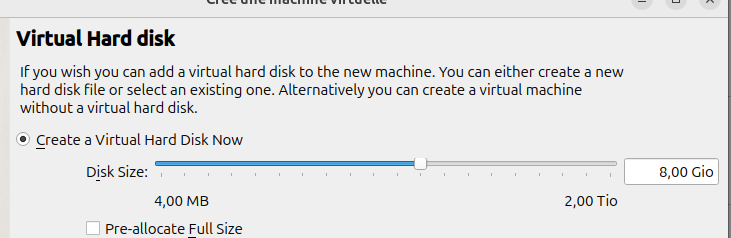
\includegraphics[scale=0.5]{./ressource/VM_Create_3.png}
\end{center}

\begin{enumerate}[resume]
\item Vous devez avant de valider avoir une configuration proche de celle présentée ci-dessous : 
\end{enumerate}


\begin{center}
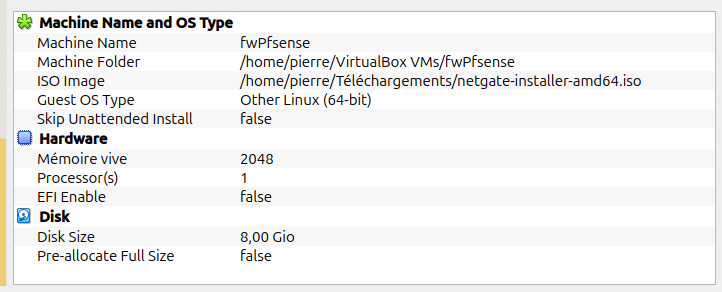
\includegraphics[scale=0.5]{./ressource/VM_Create_4.png}
\end{center}


\paragraph{La configuration physique de la machine est terminée}, il est nécessaire de configurer le réseau : 


\begin{center}
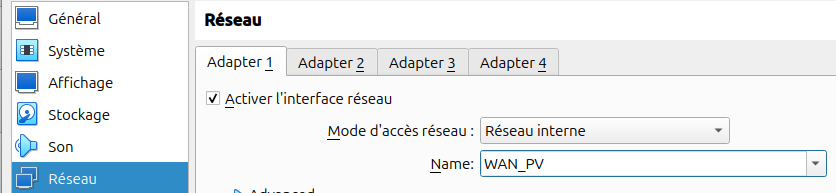
\includegraphics[scale=0.5]{./ressource/VM_network1.png}
\end{center}
\begin{center}
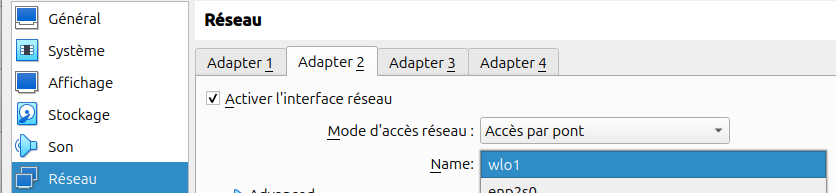
\includegraphics[scale=0.5]{./ressource/VM_network2.png}
\end{center}

\begin{center}
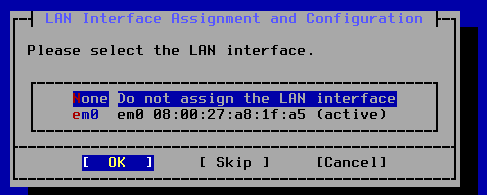
\includegraphics[scale=0.5]{./ressource/VM_network3.png}
\end{center}

\paragraph{Une fois cette opération terminée,} vous pouvez lancer la machine.

\begin{center}
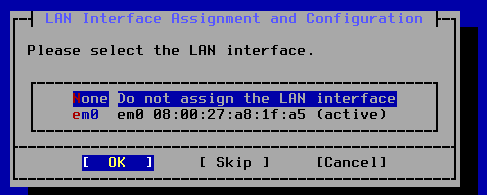
\includegraphics[scale=0.5]{./ressource/VM_network4.png}
\end{center}

\begin{center}
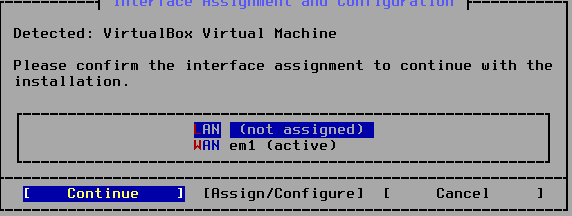
\includegraphics[scale=0.5]{./ressource/VM_network5.png}
\end{center}

\begin{center}
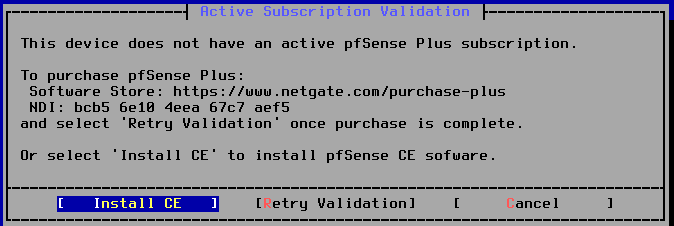
\includegraphics[scale=0.5]{./ressource/VM_network6.png}
\end{center}

\begin{center}
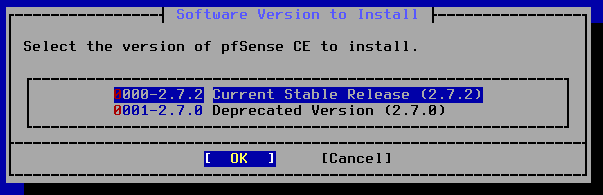
\includegraphics[scale=0.5]{./ressource/VM_network7.png}
\end{center}

Une fois l'installation terminée, la configuration du réseau va changer. Pour avoir le LAN connecté à Internet, il faut éteindre la machine et configurer les interfaces de la même manière que ci-dessous. 

\begin{center}
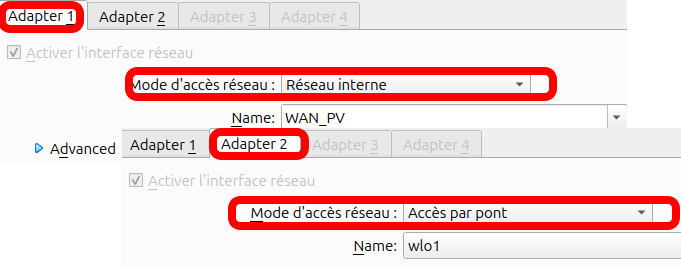
\includegraphics[scale=0.7]{./ressource/VM_finReseau0}
\end{center}
 
 Après avoir redémarré la VM, configurer l'interface LAN pour qu'elle obtienne une adresse IP via le DHCP de votre réseau (sélectionner 2 du menu puis suivre les instructions).  

\begin{center}
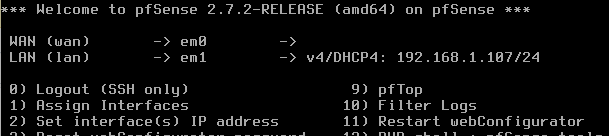
\includegraphics[scale=0.7]{./ressource/VM_finReseau1}
\end{center}
\end{document}
